% Operating-envelope figure: dynamic ratio R and surge ratio f_n/f_cam
% versus engine speed, with pass-criterion lines and the design point.
% Data from Table (rpm sweep) in Section res-envelope. No invented values.
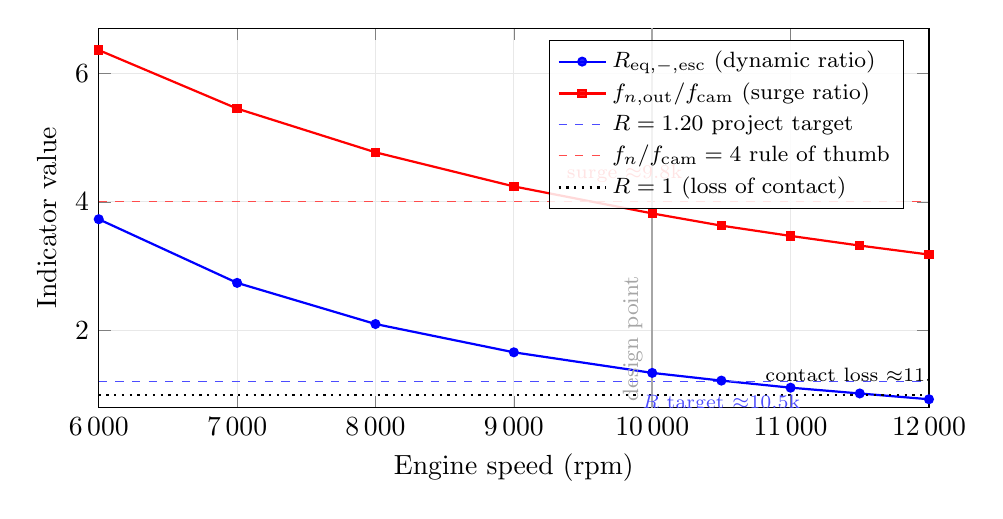
\begin{tikzpicture}
\begin{axis}[
    width=\linewidth, height=6.4cm,
    xlabel={Engine speed (rpm)},
    ylabel={Indicator value},
    xmin=6000, xmax=12000,
    ymin=0.8, ymax=6.7,
    legend pos=north east,
    legend cell align=left,
    legend style={font=\footnotesize, fill opacity=0.85, text opacity=1},
    grid=both, grid style={gray!18},
    xtick={6000,7000,8000,9000,10000,11000,12000},
    scaled x ticks=false,
    x tick label style={/pgf/number format/.cd, 1000 sep={\,}, fixed},
]
% dynamic ratio R (exhaust side, with rocker) -- blue
\addplot[thick, blue, mark=*, mark size=1.4pt] coordinates {
  (6000,3.73)(7000,2.74)(8000,2.10)(9000,1.66)(10000,1.34)(10500,1.22)(11000,1.11)(11500,1.02)(12000,0.93)};
\addlegendentry{$R_{\mathrm{eq},-,\mathrm{esc}}$ (dynamic ratio)}
% surge ratio f_n,out / f_cam -- red
\addplot[thick, red, mark=square*, mark size=1.3pt] coordinates {
  (6000,6.36)(7000,5.45)(8000,4.77)(9000,4.24)(10000,3.82)(10500,3.63)(11000,3.47)(11500,3.32)(12000,3.18)};
\addlegendentry{$f_{n,\mathrm{out}}/f_{\mathrm{cam}}$ (surge ratio)}
% pass-criterion lines
\addplot[dashed, blue!70] coordinates {(6000,1.20)(12000,1.20)};
\addlegendentry{$R=1.20$ project target}
\addplot[dashed, red!70] coordinates {(6000,4.0)(12000,4.0)};
\addlegendentry{$f_n/f_{\mathrm{cam}}=4$ rule of thumb}
\addplot[dotted, black, thick] coordinates {(6000,1.0)(12000,1.0)};
\addlegendentry{$R=1$ (loss of contact)}
% design point 10,000 rpm
\draw[gray!70, thick] (axis cs:10000,0.8) -- (axis cs:10000,6.7);
\node[gray!70, font=\footnotesize, anchor=south east, rotate=90] at (axis cs:10000,3.0) {design point};
% boundary markers
\node[red!70, font=\scriptsize, anchor=south] at (axis cs:9800,4.15) {surge $\approx$9.8k};
\node[blue!70, font=\scriptsize, anchor=north] at (axis cs:10500,1.15) {$R$ target $\approx$10.5k};
\node[black, font=\scriptsize, anchor=south] at (axis cs:11500,1.05) {contact loss $\approx$11.5k};
\end{axis}
\end{tikzpicture}
